\documentclass[__main__.tex]{subfiles}

\begin{document}

\qtitle{О}{18}
Электромагнитные волны в вакууме. Соотношение между $\vec{E}$ и $\vec{B}$ в бегущей электромагнитной волне, связь интенсивности с объёмной плотностью энергии.\\ 

Процесс распространения электромагнитного поля в пространстве называется электромагнитной волной. 

\begin{definition}
Вектор $\vec{k} = \frac{\omega}{V} \vec{n}$, где $\vec{n}$ - единичный вектор распространения волны, $V$ - скорость распространения волны, называется \textbf{волновым вектором}.
\end{definition}


\begin{enumerate}
\item
Электромагнитная волна поперечна, колебания векторов $E$ и $B$ проходят перпендикулярно направлению распространения волны (см. Рис. 80);
\item
Электрическое и магнитное поля в бегущей волне изменяются в одной фазе;
\item
Вектора $\vec{E}$,$\vec{B}$ и $\vec{V}$ (а вместе с ним и $\vec{k}$) в бегущей электромагнитной волне образуют так называемую правую тройку векторов.
\end{enumerate}

\begin{figure}[h]
\begin{minipage}{.45\linewidth}
    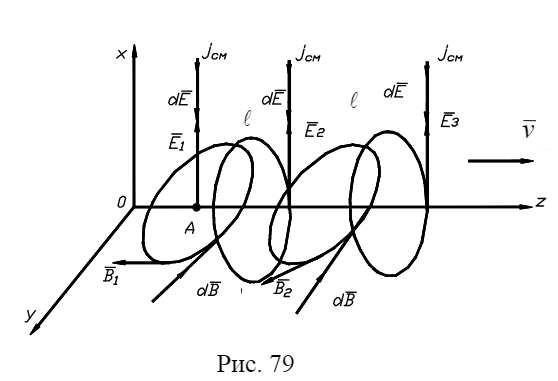
\includegraphics[width=1\linewidth]{e02_1}
\end{minipage}
\hfill
\begin{minipage}{.45\linewidth}
    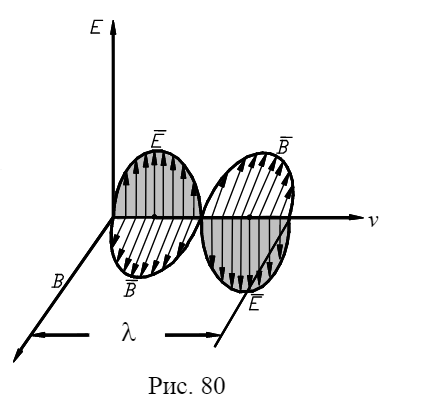
\includegraphics[width=1\linewidth]{e02_2}
\end{minipage}
\end{figure}

\textbf{Связь интенсивности с объемной плотностью энергии}

Объемная плотность энергии: $W = \frac{E^2 + B^2}{2}$

Интенсивность:
$$
I=\left<|\vec{S}|\right>=\left<W\right>v=\left<W\right>.
$$

\end{document}